\subsection{External Interface Requirements}
In the following section we list and describe the interfaces that will be provided by the software to external systems and users in order to access its functionalities. This includes user interface mockups as well as a definition of the APIs that will be realized for third party usage.

\subsubsection{User Interface}
A subset of the possible user interfaces that our platform offers to the customers is here provided. As always we divide the interfaces according to the system in examination:

\begin{itemize}
	\item Data4Help was designed to be mainly a web application. The structure of each page should be intuitive and user friendly, so that even the less experienced user in web browsing can easily use the system.
	The web interface is provided not only for the users, but also to third parties in order to better keep tracks or requests status and visualize data. A parallel API is also offered to third parties, which is described in later sections.
	\item AutomatedSOS and Track4Run are designed to be mobile applications. The following mockups show examples of the typical situations in which the user could find himself after installing the application and using it on his smart-phone. Hereunder mockups for other smart-devices are not included, but the user interfaces will be very similar to these ones. 
\end{itemize}

An example of UI mockups can be found here below.

\FloatBarrier
\graphicspath{ {../Mockups/} }

% Data4Help Mockups

% User

\begin{figure}
  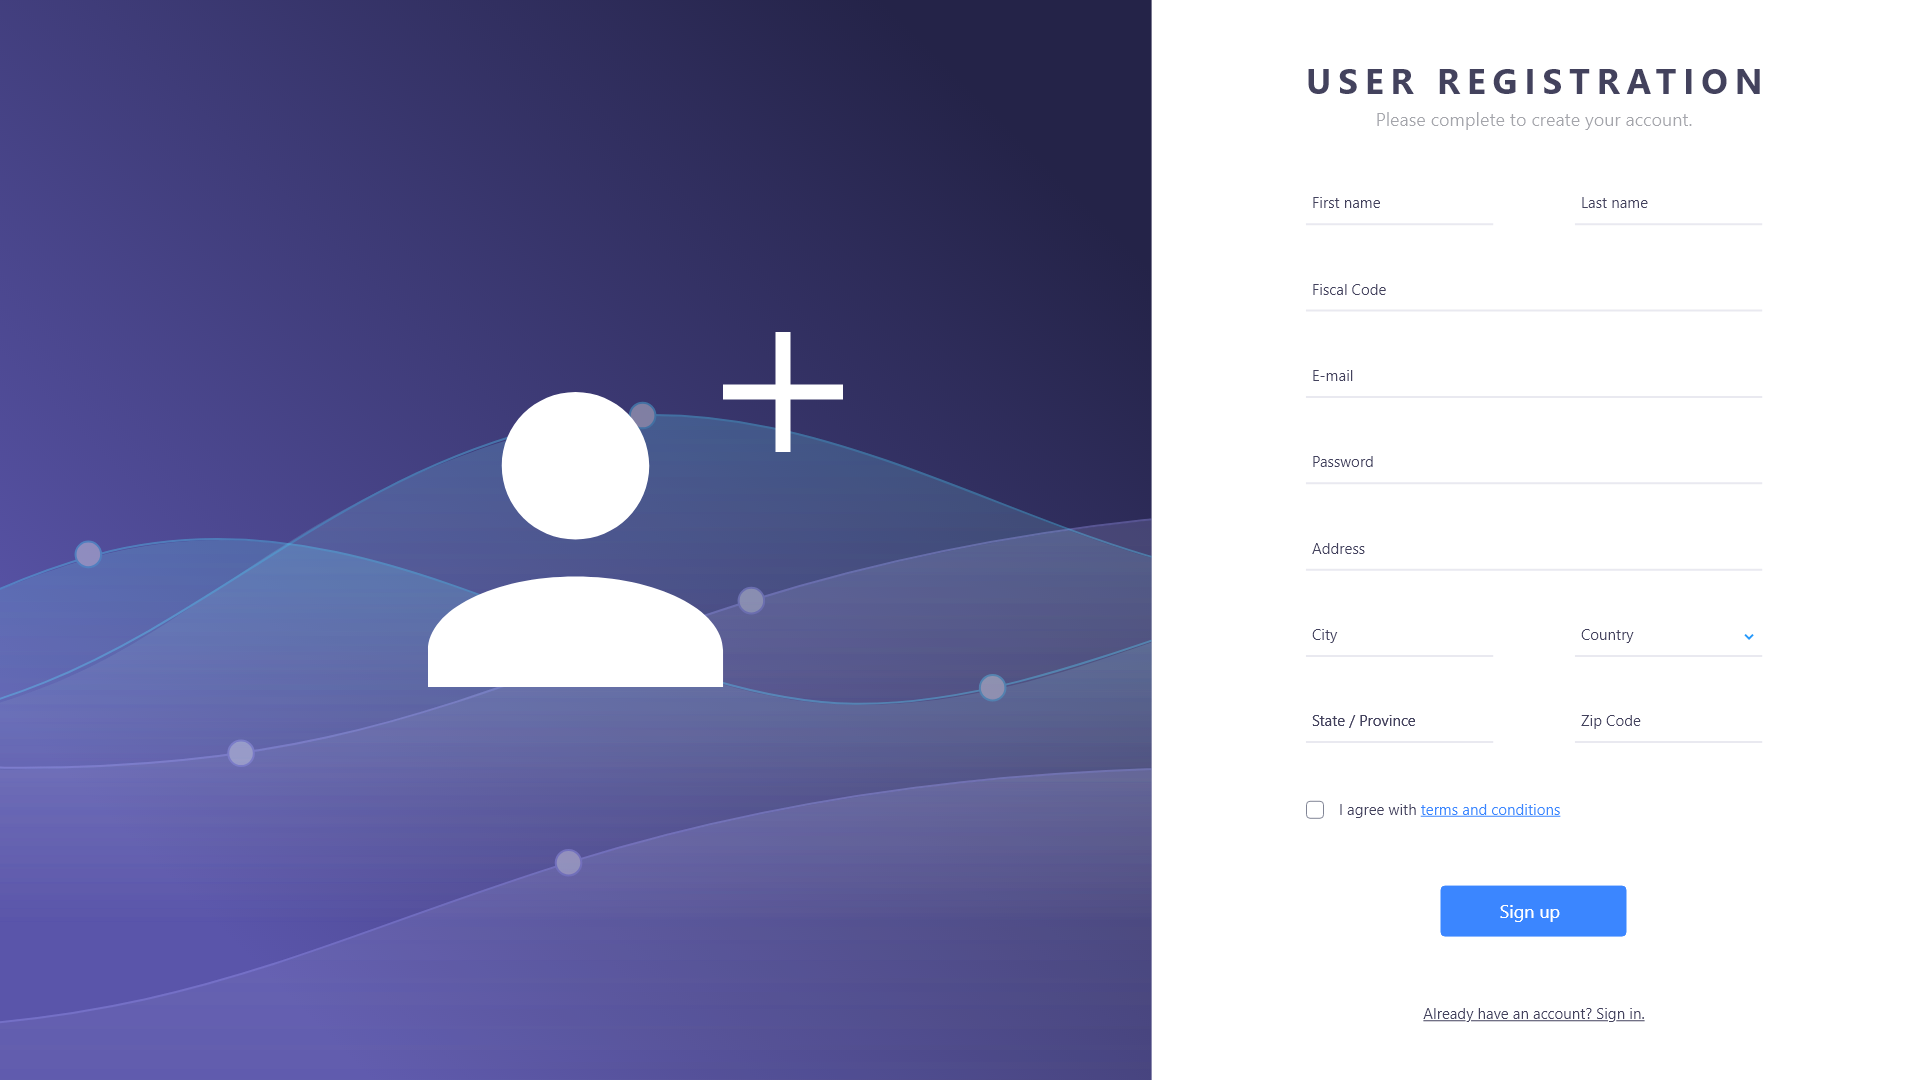
\includegraphics[width=\linewidth]{Data4Help/userRegistration.png}
  \caption{Data4Help - User Registration}
  \label{Data4Help - User Registration}
\end{figure}

\begin{figure}
  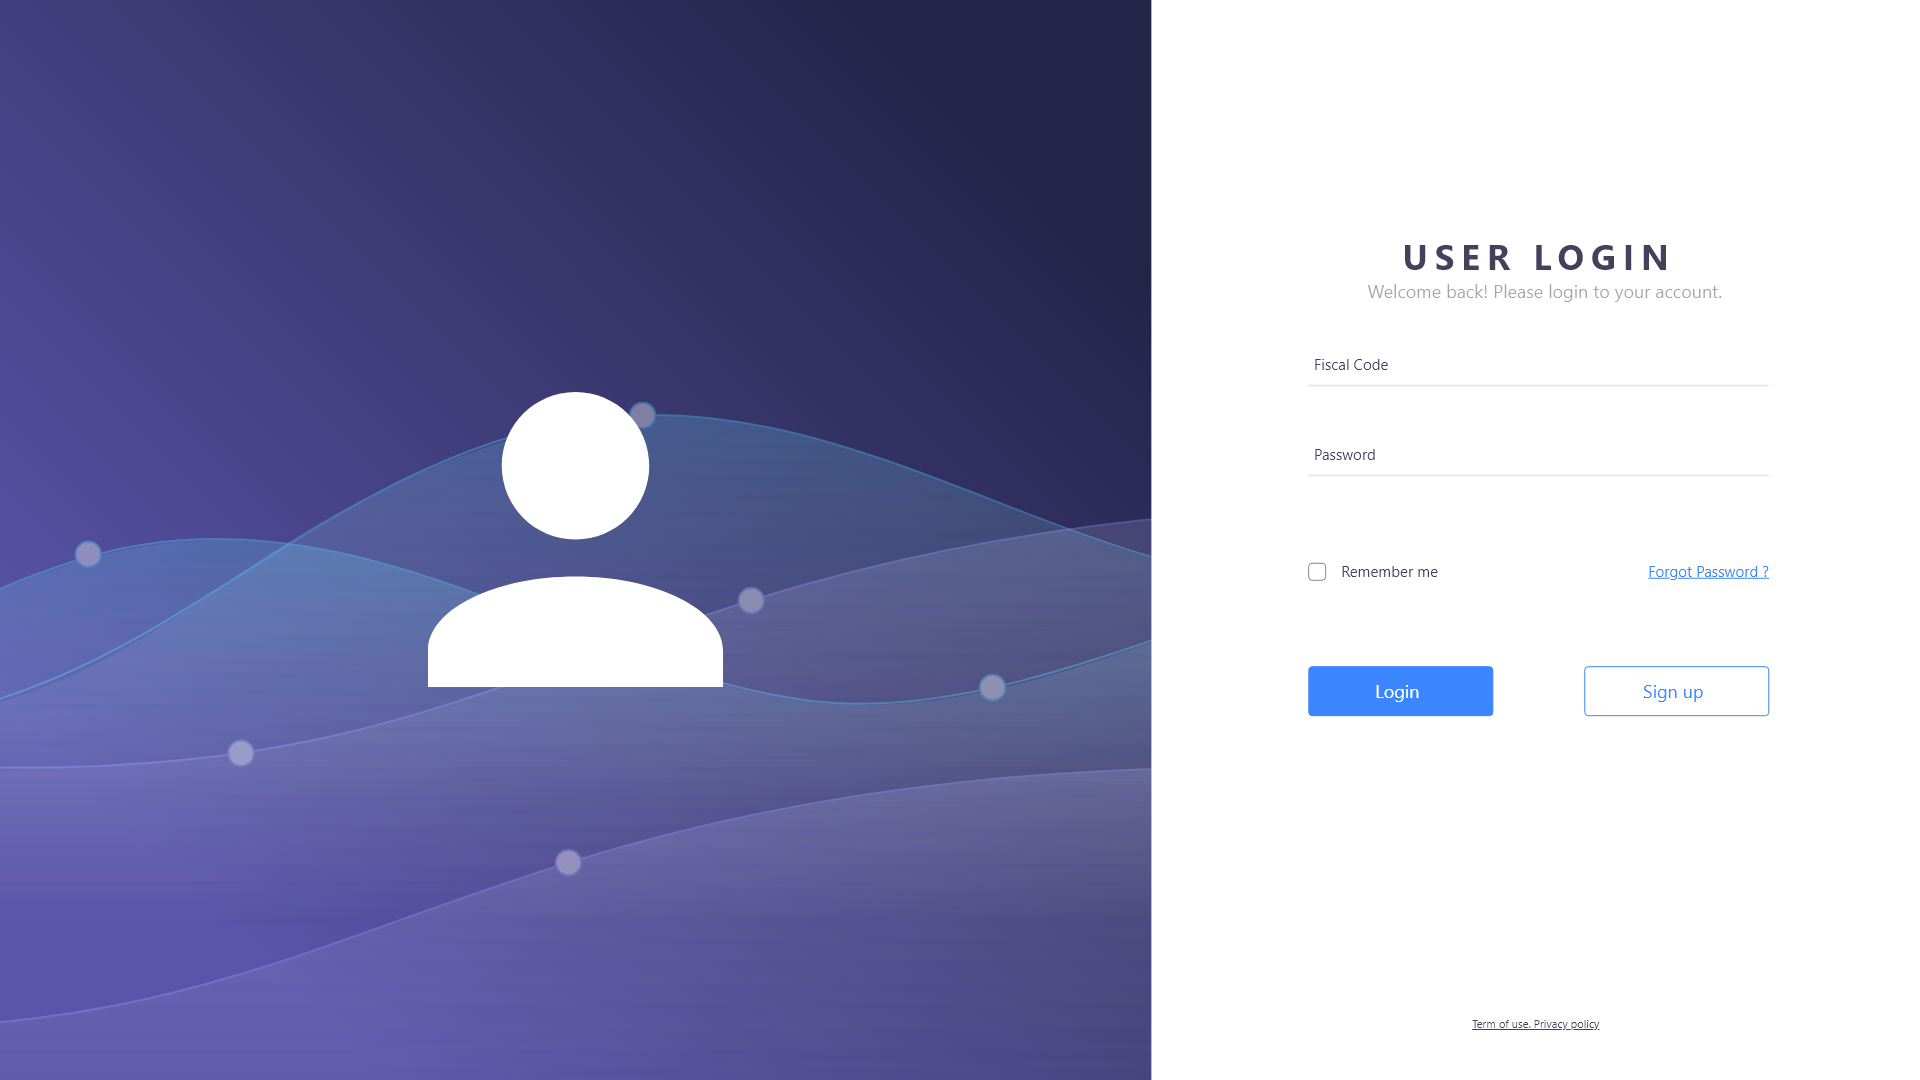
\includegraphics[width=\linewidth]{Data4Help/userLogin.png}
  \caption{Data4Help - User Login}
  \label{Data4Help - User Login}
\end{figure}

\begin{figure}
  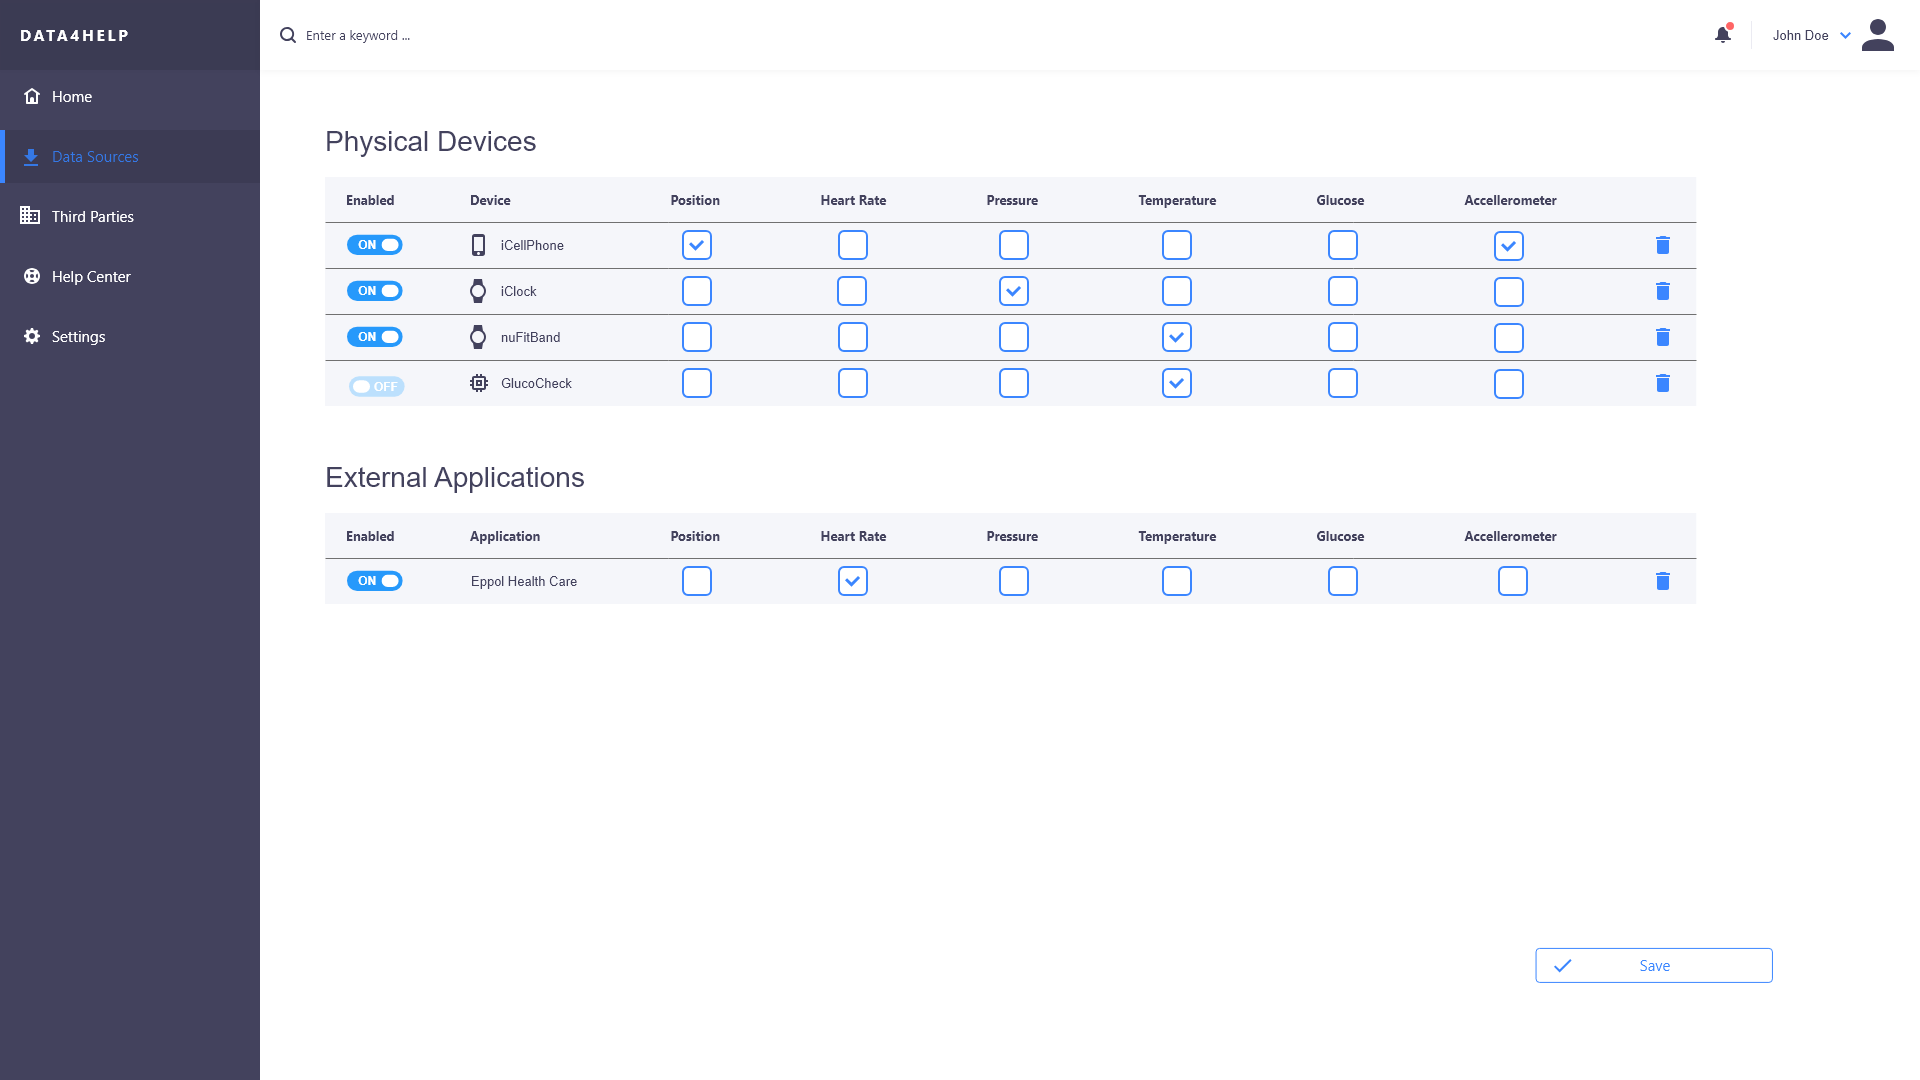
\includegraphics[width=\linewidth]{Data4Help/userDataSources.png}
  \caption{Data4Help - User Data Sources Management}
  \label{Data4Help - User Data Sources Management}
\end{figure}

\begin{figure}
  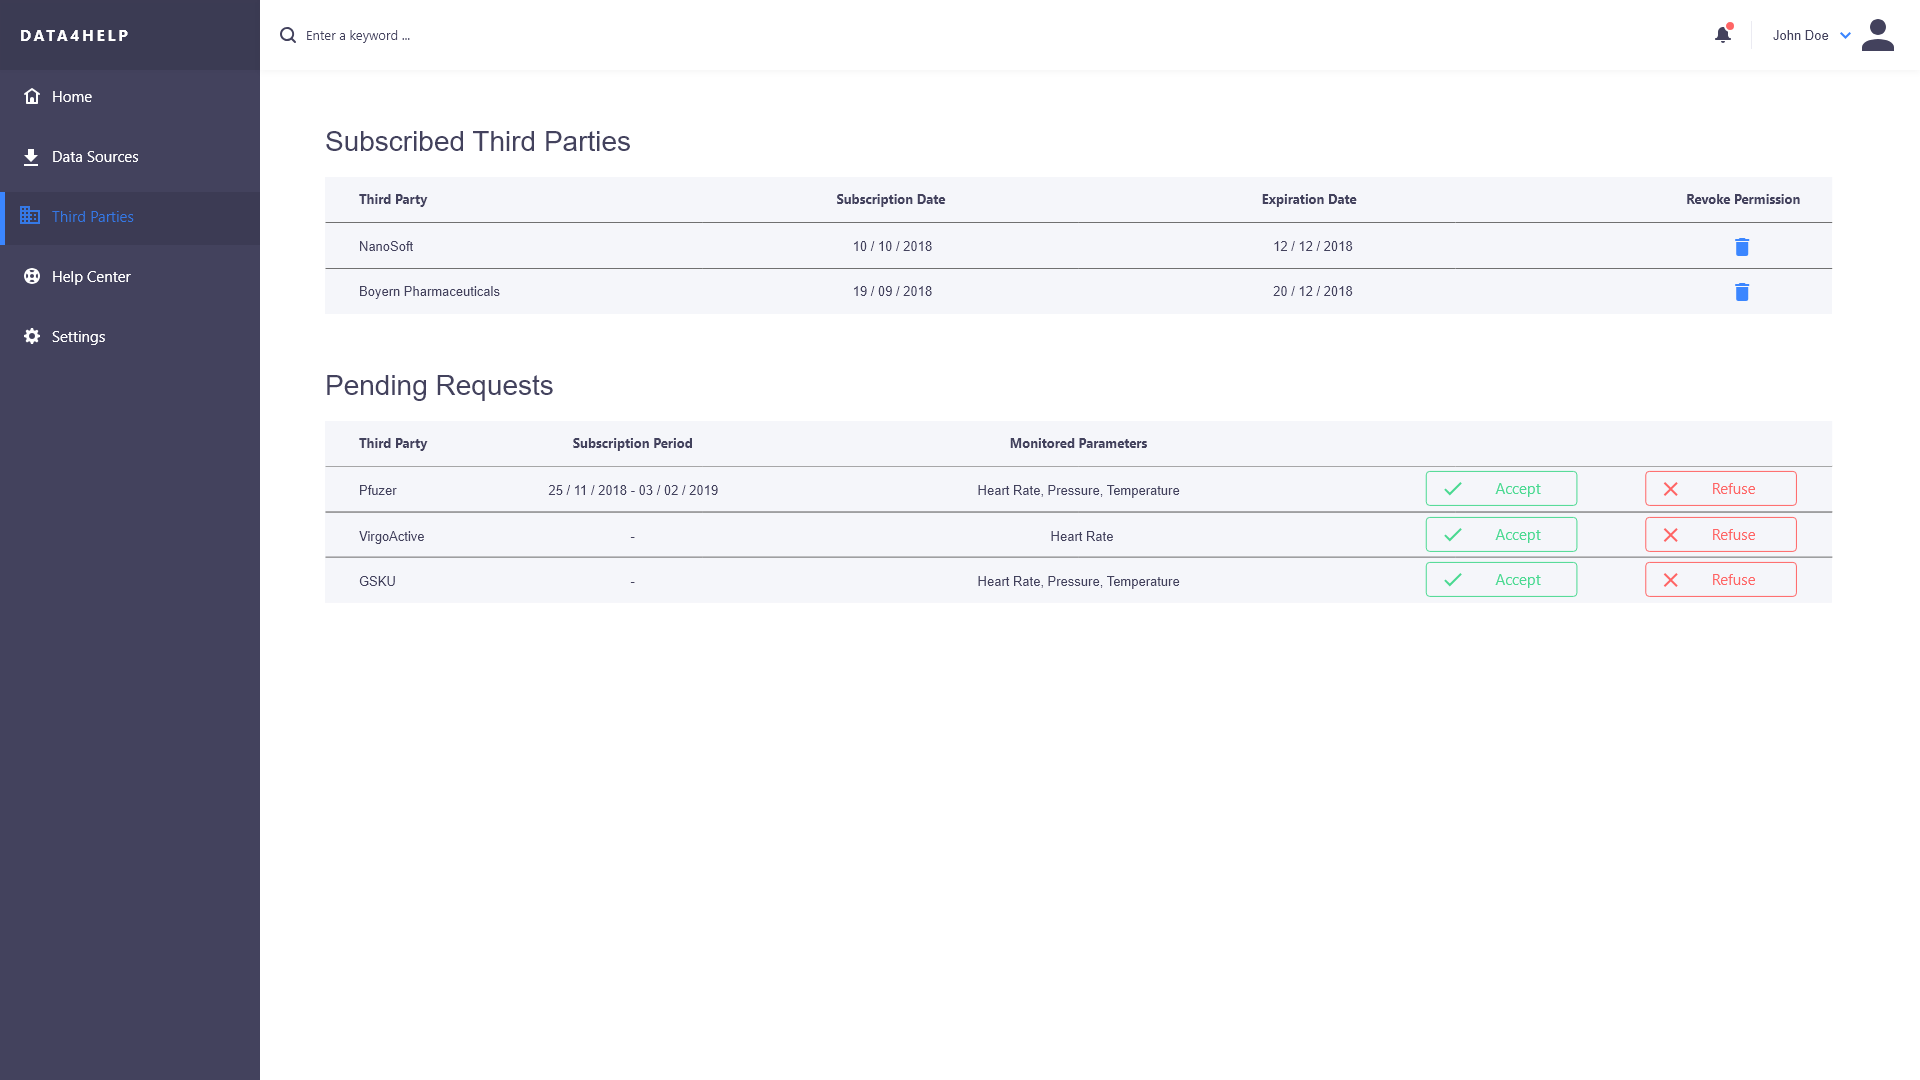
\includegraphics[width=\linewidth]{Data4Help/userThirdPartiesManagement.png}
  \caption{Data4Help - User Third Parties Management}
  \label{Data4Help - User Third Parties Management}
\end{figure}

% Third Parties

% AutomatedSOS Mockups

\begin{figure}[!ht]
  \centering
  \begin{subfigure}[b]{0.4\linewidth}
    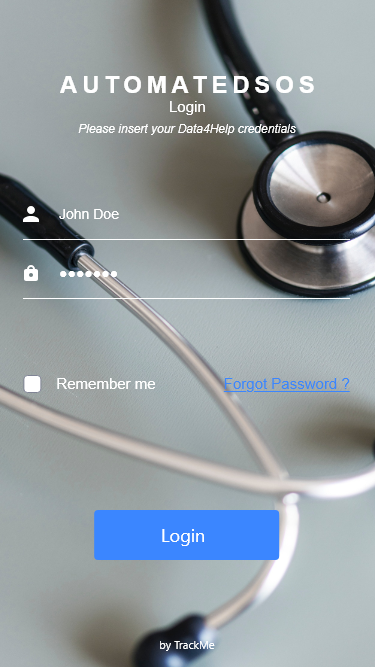
\includegraphics[width=\linewidth]{AutomatedSOS/Login.png}
    \caption{Login}
  \end{subfigure}\hfill
  \begin{subfigure}[b]{0.4\linewidth}
    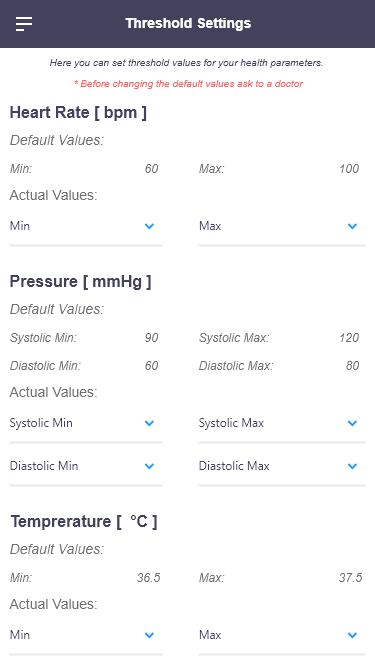
\includegraphics[width=\linewidth]{AutomatedSOS/thresholdSettings.png}
    \caption{Threshold Settings}
  \end{subfigure}
  \par\bigskip
  \begin{subfigure}[b]{0.4\linewidth}
    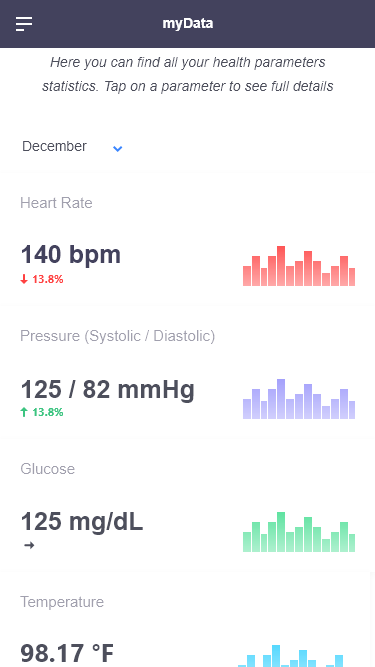
\includegraphics[width=\linewidth]{AutomatedSOS/myData.png}
    \caption{myData}
  \end{subfigure}\hfill
  \begin{subfigure}[b]{0.4\linewidth}
    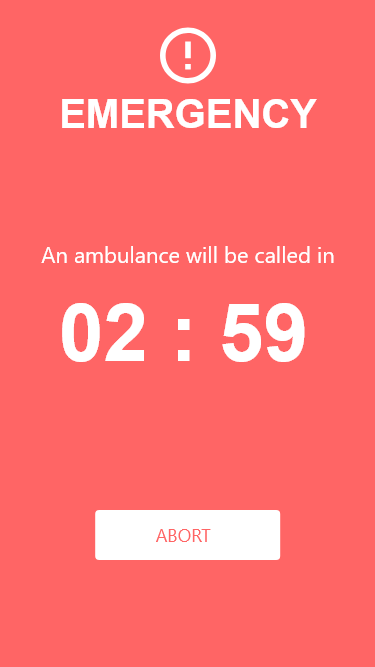
\includegraphics[width=\linewidth]{AutomatedSOS/emergencyAlert.png}
    \caption{Emergency Alert}
  \end{subfigure}
  \caption{AutomatedSOS Mockups}
\end{figure}

% Track4Run Mockups

\begin{figure}[!ht]
  \centering
  \begin{subfigure}[b]{0.4\linewidth}
    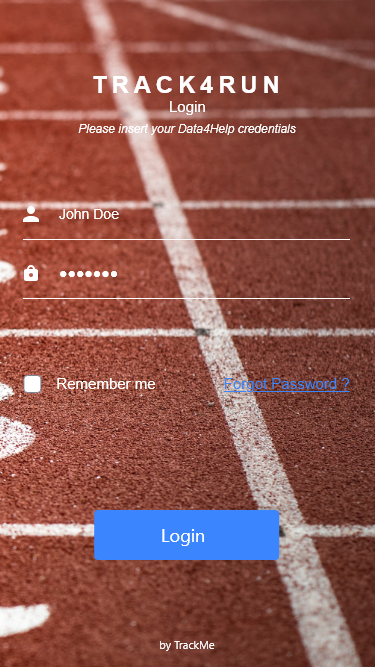
\includegraphics[width=\linewidth]{Mockups/Track4Run/Login.png}
    \caption{Login}
  \end{subfigure}\hfill
  \begin{subfigure}[b]{0.4\linewidth}
    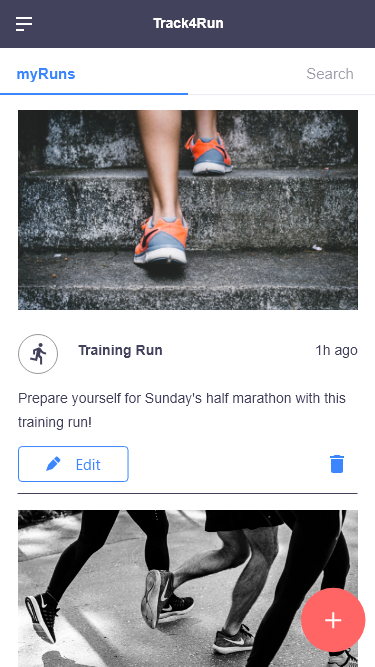
\includegraphics[width=\linewidth]{Track4Run/myRuns.png}
    \caption{myRuns}
  \end{subfigure}
  \par\bigskip
  \begin{subfigure}[b]{0.3\linewidth}
    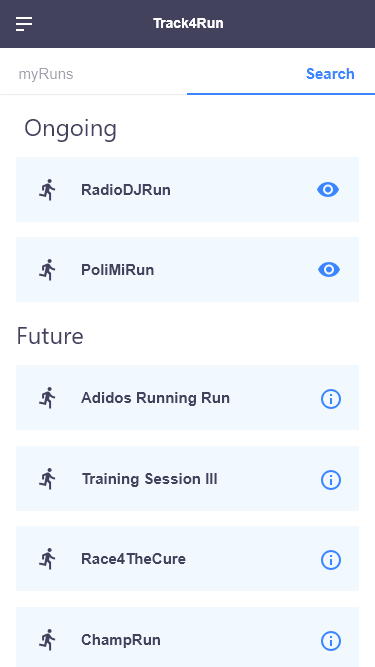
\includegraphics[width=\linewidth]{Track4Run/Search.png}
    \caption{Search}
  \end{subfigure}\hfill
  \begin{subfigure}[b]{0.3\linewidth}
    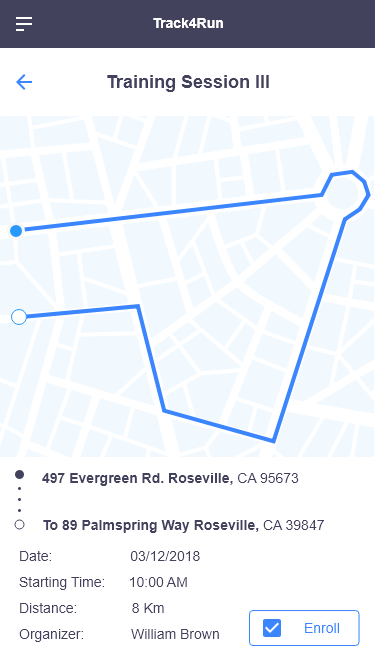
\includegraphics[width=\linewidth]{Track4Run/InfoMap.png}
    \caption{Run Details}
  \end{subfigure}\hfill
  \begin{subfigure}[b]{0.3\linewidth}
    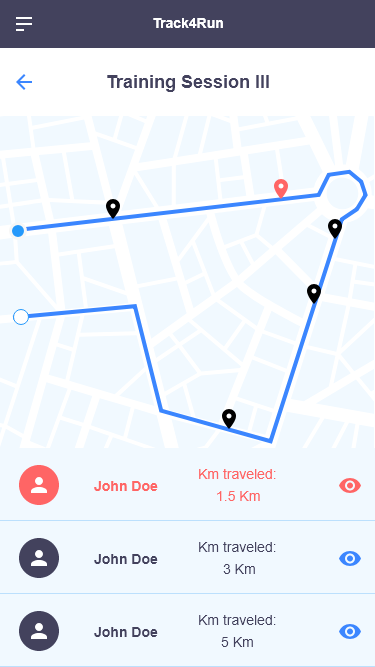
\includegraphics[width=\linewidth]{Track4Run/InfoMapMarked.png}
    \caption{Live Run Details}
  \end{subfigure}
  \caption{Track4Run Mockups}
\end{figure}
\FloatBarrier

\subsubsection{Hardware Interfaces}
Since our system is designed to be a software platform running on any compatible hardware, no proprietary hardware interface is provided.

\subsubsection{Software Interfaces}
The main external software interfaces of our system can be found in Data4Help, which as already explained is the part responsible of connecting data producers to data consumers.
To achieve this goal, Data4Help exposes two main software interfaces, which can be thought as APIs that are given to the third party applications in order to connect their software to ours.

\begin{itemize}
	\item \textbf{Data Sharing Interface:} this interface can be used from third party organizations that want to access the user data contained in the system.
	The interface shall offer four main functionalities: authentication, group data requests, single data requests, subscription requests.
	
	Authentication must be done using a trustful way of identifying the organization that wants to register to the system, in order to prevent malicious actors to infiltrate the system. This can be for example an electronic signature connected with the VAT code of the company.
	
	Group data and single user data requests are defined by some filters that the third party wants to apply in order to retrieve only the needed data, and when this is possible they will generate a response containing the latest available data from the system.
	
	 Finally, subscription to new data can be performed by providing a callback interface, that will then be notified with some specific call whenever some new data is available on the system.
	 
	\item \textbf{Data Acquisition Interface:} this interface is provided to the applications and hardware devices that collect data from the user, and gives the possibility to add this kind of information to the user's data set in the system.
	
	As for third parties, authentication is necessary in this case too. This can be provided by the data source using the user's Data4Help credentials, so that the systems knows which user is adding that data source.
	
	Once authenticated, the data source is provided with an interface to send data streams to the Data4Help system, that will collect and store them safely. 
\end{itemize}

\subsubsection{Communication Interfaces}
As communication interfaces, this system will use the commonly available protocols to access the internet and to make remote calls to software interfaces of external and internal systems.

\subsection{Functional Requirements}

\subsubsection{Requirements}
\textbf{[G1] Data4Help must be able to keep track of real time health status and position from registered users' devices}
\begin{itemize}
	\item \textbf{[R1]} A User shall be able to register to TrackMe's services providing a Fiscal code and a password of their choice
	\item \textbf{[R2]} A User shall be able to unsubscribe from the service at any moment
	\item \textbf{[D1]} Fiscal code uniquely identifies a user of the system
	\item \textbf{[R3]} After registration, a user must be able to log in by using his/her credentials
	\item \textbf{[R4]} The system must acquire user data only after he/she accepted the data acquisition policy
	\item \textbf{[R5]} The system shall acquire data from external applications that register themselves as data sources of a user
	\item \textbf{[D2]} Every user owns at least one device capable of retrieving correct real-time health parameters and location
	\item \textbf{[D3]} User devices must grant to the system access to the requested data
	\item \textbf{[D4]} User devices must be continuously connected to the internet
\end{itemize}

\textbf{[G2] Data4Help should allow third parties to gather information from a single user or from an anonymous group of users}
\begin{itemize}
	\item \textbf{[R6]} Third parties must be able to register to Data4Help by providing a VAT code
	\item \textbf{[D5]} VAT code uniquely identifies a third party in the system
	\item \textbf{[R7]} The system shall provide to the registered third parties unique access tokens to use the services
	\item \textbf{[R8]} The system must grant access to a single user data only after his/her confirmation
	\item \textbf{[D6]} Third parties know the monitored user Fiscal Code
	\item \textbf{[R9]} The system must be capable of merging multiple user data and anonymize it
	\item \textbf{[R10]} The system shall grant access to merged data only if the number	of individuals	whose data satisfy the request is higher than	 1000
\end{itemize}

\textbf{[G3] Data4Help should allow third parties to subscribe to new data and receive them as soon as they're produced}

\begin{itemize}
	\item \textbf{[R11]} The system must store information about third parties' data subscriptions
	\item \textbf{[R12]} The system asks to the third parties who want to subscribe to new data to provide a callback interface
	\item \textbf{[D7]} Third parties are able to provide callback interfaces
	\item \textbf{[R13]} The system must notify every observing third party through their callbacks whenever an observed data changes
	\item \textbf{[R14]} The system must provide an interface to start and manage requests
	\item \textbf{[R15]} The system must give the possibility to third parties to unsubscribe from user data
\end{itemize}

\textbf{[G4] AutomatedSOS should be able to identify an health emergency when the user data are below/exceeding a certain threshold}
\begin{itemize}
	\item \textbf{[R16]} AutomatedSOS users must be signed in with a Data4Help account
	\item \textbf{[R17]} AutomatedSOS can use data coming from Data4Help to monitor the health condition of its users
	\item \sout{\textbf{[R18]} AutomatedSOS, when possible, uses data coming directly from the device sensors.}
	\item \textbf{[R19]} When activated, AutomatedSOS provides some default values for parameters thresholds
	\item \textbf{[R20]} AutomatedSOS gives the user the possibility to set his/her own threshold 
	\item \textbf{[D8]} AutomatedSOS has access to parameters that can be useful for identifying an emergency status
	\item \textbf{[R21]} AutomatedSOS shall be able to unsubcribe from the service at any time
\end{itemize}

\textbf{[G5] AutomatedSOS must notify the user and call an ambulance when it detects a health emergency}
\begin{itemize}
	\item \textbf{[D9]} There exists an API through which AutomatedSOS can pass to an ambulance information about the identity, the location and the vital parameters of the person in trouble
	\item \textbf{[R22]} The system must notify the user before calling the ambulance
	\item \textbf{[R23]} The system gives the possibility to abort the operation within 5 seconds
	\item \textbf{[R24]} The system automatically calls the ambulance if the operation is not aborted
\end{itemize}

\textbf{[G6] Track4Run allows an organizer to create and manage a run.}
\begin{itemize}
	\item \textbf{[R25]} Track4Run users must be signed in with a Data4Help account
	\item \textbf{[R26]} Track4Run allows organizers to create a "run event" providing the track, the date and a starting and ending time
	\item \textbf{[R27]}  Track4Run allows organizers to modify the details of the created event
	\item \textbf{[R28]} Track4Run allows organizers to delete his created runs
	\item \textbf{[R29]} Track4Run gives the possibility to the organizers to extend editing permissions of an event to other users (co-organizers) 
	\item \textbf{[R30]} Track4Run can show to an organizer a list of his past, ongoing and future events
\end{itemize}

\textbf{[G7] Track4Run allows a user to partecipate to an organized run}
\begin{itemize}
	\item \textbf{[D10]} Track4Run athlete wears the monitoring device during the whole run
	\item \textbf{[R31]} Track4Run gives the user the possibility to look up for future organized runs and join them
	\item \textbf{[R32]} Track4Run gives the user the possibility to unsubscribe from a previously joined run at any moment
	\item \textbf{[R33]} Track4Run must keep track of the position of every participant of the run from the start until the end of the event
\end{itemize}

\textbf{[G8] Track4Run allows a spectator to track the position of the partecipants of the run}
\begin{itemize}
	\item \textbf{[R34]} Track4Run gives the spectator the possibility to look up for ongoing runs and select the one to follow
	\item \textbf{[R35]} Track4Run shows to the spectator the position of all the participants of the selected run on a map
	\item \textbf{[D11]} There is system providing an API to visualize GPS data on a map.
\end{itemize}
 
\subsubsection{Scenarios}
\textbf{Scenario 1}
While talking, John tells his friend Matt about a new web service called Data4Help that helps you keeping track of your health status. Hence Matt, interested in checking his heart rate, decide to register to it. In order to do this he has to fill a form with his personal information, including his fiscal code, and choose a username and password  that will be used as credentials for the login. 
After filling the form he clicks on the final checkbox to accept the terms and conditions and complete his registration.
Thereafter Matt receives a notification saying he has registered successfully to Data4Help.
\\
\\
\textbf{Scenario 2}
Mary, a Data4Help customer, received for her birthday the new Eppol iClock. Knowing that Eppol's products support Data4Help data soure synchronization, she decide to pair her new device with her Data4Help account. She searches for this feature in her iClock and enables it.
Soon a confirmation request arrives via email and she confirms it. The device is added to the already available data sources.
After that Mary goes on Data4Help webpage, logs in, browse to the "Data Sources" section and sees the new iClock between the available sources. There she assigns the tracking of the "Hearth Rate" parameter to her smartwatch. With the same procedure, she assigns to her smartphone the tracking of the "Position" parameter.
She's then satisfied with her preferences and saves them.
\\
\\
\textbf{Scenario 3}
Michael Garcia, Boyer Pharmaceutical CEO, heard about the Data4Help service and in agreement with the Administrative Board, he decided to introduce it in the company. He visits  www.data4help.com/ and clicks on the "Business" section in order to register his company as a registered third party of the service. To do this, Michael fills in the registration form with all the requested information about the company, including the VAT Code and the Electronic Signature, and confirms it. A confirmation allert is immediatly show saying the registration procedure has been successfully completed.
\\
\\
\textbf{Scenario 4}
Brian, patient of the Lenox Private Medical Center, was released  yesterday. The clinic, registered to the Data4Help service, decides to monitor his health status to see if the treatment he was under reached the desired results.
The doctor that was in charge of Brian logs in to the Data4Help reserved page of the clinic. Once logged in he goes under the "Requests" tab. There, with the aid of many checkboxes, he craft a request to monitor Brian's data.
As soon as the doctor sends the request, Brian receives an email notification. He then accept the request, clicking the link in the email. The Lenox Private Medical Center is added to the Third Party Management list on Brian's account. A confirmation email, saying that the user accepted the request is sent to the Medical Center. 
The doctor sees the e-mail and goes in the "Requests" section of the Data4Help personal page of the company, and from there to the accepted ones. After clicking on Brian's answer, all the requested data are displayed on screen.
\\
\\
\textbf{Scenario 5}
Pfuzer, a big pharmaceutical company registered to Data4Help service, needs to gather the heart rate data of all the italian young people under 30 years old for a market analysis aimed at evaluating the production of a new drug against heart disease. For this reason Todd Chavez, the marketing manager of the company, goes to the Pfuzer personal Data4Help page and once logged  in he clicks on the "Requests" tab in the home page. Once in the page he fills a form, filtering the location of the search. Then he tries to send the request but a warning message is immediately displayed on screen saying that the request cannot be satisfied. For this reason, Todd decides to untighten the search parameters. After changing them, the constraints are satisfied and the requested data is immediately made available under the Accepted tab.
\\
\\
\textbf{Scenario 6}
Andrew decided to buy the new iClock as a gift for the birthday of his grandfather Leonard, 93
years old, who suffers from severe heart problems and lives alone. Since Leonard would like to be autonomous, his new device with AuotmatedSOS service active on it, grants him a safer life.

One night Leonard wakes up with severe chest pains. The iClock immediately detects the "heart rate" parameter exceeded the maximum threshold and shows a noisy emergency alert, saying that an ambulance will be called if the user doesn't abort in the following minute. Leonard is really sick and is not able to abort the operation. In few minutes an ambulance arrives and Leonard is immediately rescued.
\\
\\
\textbf{Scenario 7}
William suffers from epilepsy. The attacks are not very frequent but they are so strong that a few months ago he fell and he got a nasty head injury. While looking for an automated solution to check on his conditions, he hears about AutomatedSOS and decides to activate the service provided by Data4Help.

At first he sets the threshold of the tracked parameters with the help of his doctor and he adds the contacts of his parents. When the wristwatch detects repetitive shaking motion, it automatically sends the user’s bluetooth-connected phone text and call alerts to the designated recipients. Within seconds, family members receive these alerts, which include the date, time and GPS location of the event.
\\
\\
\textbf{Scenario 8}
Steve, a AutomatedSOS customer with diabete, needs to periodically check the glucose levels observed by his medical device connected with the AutomatedSOS application on his smartphone. For doing this, he starts the application and goes on the "myData" tab. A nice view appears, containing all the information about his monitored health parameters with a lot of colorful diagrams. Steve filters out the displayed content by selecting the desired observation period. He's then presented with all the data gathered for that period. 
\\
\\
\textbf{Scenario 9}
Mario is a personal trainer and he is organizing a run for all his athletes. He is thinking about using the Track4Run Service to accomplish this task. So he download the Track4Run application and logs in with his Data4Help credentials. Once the application is installed and running, he goes under the "myRuns" section and taps on the big plus button. 

At this point a configuration frame shows up. Luke starts by filling out a form: he adds the event name, the travelled distance and the starting and ending time. Finally, by clicking on a map, he marks all the checkpoints of the run.

After a quick check, Luke clicks on the "Create" button and a confirmation alert appears saying that the event has been successfully published in the news feed.
\\
\\
\textbf{Scenario 10}
Chris, runner and Data4Help customer, is looking for a run to join. By looking at the  news feed of Track4Run on his smartphone he sees the event created by Mario. He taps on the event name and the full description of the event shows up. After reading the description and all the details he decides to join the run, hence he clicks on the "Participate" button. A confirmation alert shows up, saying that the event has been added to the attending events.
\\
\\
\textbf{Scenario 11}
Katy, Chris' wife and Data4Help customer,  wants to go cheer his husband at the run. The day of the run she launches the Track4Run and searches for his husband run under the "search" tab. Katy selects the desired run and a nice map with a the GPS position of all the athletes opens up.

\newpage
\subsubsection{Use Cases}

\begin{table}[h!]
\begin{tabular}{|l|p{12cm}|}
\hline
Name             & User registration \\ \hline
Actor            & User \\ \hline
Entry conditions & User enters in the Data4Help web page \\ \hline
Events flow      & \begin{enumerate}
\item Click on the "Sign Up" button
\item Fill the registration form and the account credentials
\item Accept the terms and conditions by clicking on the checkbox 
\item Click on the "Sign Up" button
\item The system elaborate the registration and send back a notification
\end{enumerate} 
\\ \hline
Exit conditions  & Registration is successful and the user is informed via notification \\ \hline
Exceptions       & \begin{enumerate}
\item The user is already registered
\item There is some invalid data in the form
\item The email is already used
\item Terms and conditions haven't been checked
\end{enumerate} All the exceptions take the user back to the registration procedure \\ \hline
\end{tabular}
\end{table}

\FloatBarrier
\begin{table}[h!]
\begin{tabular}{|l|p{12cm}|}
\hline
Name             & User Login \\ \hline
Actor            & User \\ \hline
Entry conditions & User already registered and enters Data4Help web page\\ \hline
Events flow      & \begin{enumerate}
\item Click on the "Log in" button
\item The user enter his/her credentials
\item Click on the "Enter" button
\item The log in was successful and the user is redirected to the home page of the App
\end{enumerate} \\ \hline
Exit conditions  & The log in is successful and the user is redirected to home page \\ \hline
Exceptions       & \begin{enumerate}
\item Credentials aren't valid
\end{enumerate} The exceptions are notified to the user and the Login procedure restart \\ \hline
\end{tabular}
\end{table}

\begin{table}[h!]
\begin{tabular}{|l|p{12cm}|}
\hline
Name             & Add Data Source \\ \hline
Actor            & User \\ \hline
Entry conditions & User synchronizes his device or application with Data4Help \\ \hline
Events flow      & \begin{enumerate}
\item A confirmation email is sent to the user
\item The user reads the email and clicks on the provided confirmation link
\item The data source is added to user account 
\end{enumerate} \\ \hline
Exit conditions  & The user confirms the synchronization \\ \hline
Exceptions       & \begin{enumerate}
\item The user didn't request the synchronization and doesn't click on the confirmation
\end{enumerate} After 24 hours the request is made void and a notification email 
is sent to the user \\ \hline 
\end{tabular} 
\end{table}

\newpage
\begin{table}[h!]
\begin{tabular}{|l|p{12cm}|}
\hline
Name             & Data Sources Management \\ \hline
Actor            & User \\ \hline
Entry conditions & User enter in the "Data Sources" section of the web site \\ \hline
Events flow      & \begin{enumerate}
\item The list of data sources connected to the account is shown
\item The user select which source to configure
\item For that source, the list of all the possible parameter that it can track is shown
\item The user turns On/Off the tracking of each parameter
\item Clicks on the "Save" button
\end{enumerate} \\ \hline
Exit conditions  & The user have set his/her preference and saves them \\ \hline
Exceptions       & \begin{enumerate}
\item the parameter is already tracked from a more reliable source (maybe??)
\end{enumerate} \\ \hline
\end{tabular}
\end{table}

\begin{table}[h!]
\begin{tabular}{|l|p{12cm}|}
\hline
Name             & Third Party Registration \\ \hline
Actor            & Third Party \\ \hline
Entry conditions & The third party clicks on "Business" on www.trackme.com/data4help \\ \hline
Events flow      & \begin{enumerate}
\item Clicks on the "Sign Up" button
\item Fills the form with information regarding the company
\item Clicks on the "Sign Up" button
\end{enumerate} \\ \hline
Exit conditions  & Registration is successful and the user is informed via notification \\ \hline
Exceptions       & \begin{enumerate}
\item Company already registered
\item Electronic Signature not valid
\end{enumerate} All the exceptions are notified and the procedure goes back to registration \\ \hline
\end{tabular}
\end{table}

\newpage
\begin{table}[h!]
\begin{tabular}{|l|p{12cm}|}
\hline
Name             & Third Party Login \\ \hline
Actor            & Third Party \\ \hline
Entry conditions & The third party goes on www.trackme.com/data4help and click "Login" \\ \hline
Events flow      & \begin{enumerate}
\item Click on the "Login" button
\item Enter the company credentials
\item Click on the "Login" button
\end{enumerate} \\ \hline
Exit conditions  & Login is successful and the client is redirected to its reserved page  \\ \hline
Exceptions       & \begin{enumerate}
\item Credentials are not valid
\end{enumerate} The exceptions are notified to the client and the Login procedure restart  \\ \hline
\end{tabular}
\end{table}

\newpage
\begin{table}[h!]
\begin{tabular}{|l|p{12cm}|}
\hline
Name             & One Shot Single Data Request \\ \hline
Actor            & Third Party, User \\ \hline
Entry conditions & A third party client is logged in and goes in the "Requests" section\\ \hline
Events flow      & \begin{enumerate}
\item Clicks on "New Request" button
\item Selects "Single Request" radio button
\item Selects the "One Shot" radio button
\item Inserts the fiscal code of the recipient and the request name in text fields
\item Inserts a brief description of the request by filling a text area
\item Checks which parameters to monitor from a checklist
\item Clicks on the "Send" button
\item The request is notified to the user via email
\item The user checks his email and clicks on the confirmation link
\item The result is notified via e-mail to the third party
\item If the user accepted, the information are made available under 
the "Accepted" section of the "Request" Data4Help personal page of the company
\end{enumerate} \\ \hline
Exit conditions  & The user has responded to the request and, if successful, 
the data are made available to the third company \\ \hline
Exceptions & \begin{enumerate}
\item No user found that correspond to the search
\item The user refuses the request
\end{enumerate} This exception is notified to the third party and the request ends \\ \hline
\end{tabular}
\end{table}

\newpage
\begin{table}[]
\begin{tabular}{|l|p{12cm}|}
\hline
Name             & Subscription Single Data Request \\ \hline
Actor            & Third Party, User \\ \hline
Entry conditions & A third party client is logged in and goes in the "Requests" section\\ \hline
Events flow      & \begin{enumerate}
\item Clicks on "New Request" button
\item Selects "Single Request" radio button
\item Selects the "Subscription Period" from a dropdown
\item Inserts the fiscal code of the recipient and the request name in text fields
\item Inserts a brief description of the request by filling a text area
\item Checks which parameters to monitor from a checklist
\item Clicks on the "Send" button
\item The request is notified to the user via email
\item The user checks his email and clicks on the confirmation link
\item The result is notified via e-mail to the third party
\item If the user accepted, the information are made available under the "Accepted" 
section of the "Request" Data4Help personal page of the company
\item Every time that the requested data changes in the Data4Help database, 
the data available to the third party are updated
\end{enumerate} \\ \hline
Exit conditions  & The Subscription Period ends \\ \hline
Exceptions & \begin{enumerate}
\item No user found that correspond to the search
\item The user refuses the request
\end{enumerate} This exception is notified to the third party and the request ends\\ \hline
\end{tabular}
\end{table}

\newpage
\begin{table}[h!]
\begin{tabular}{|l|p{12cm}|}
\hline
Name             & One Shot Group Data Request \\ \hline
Actor            & Third Party \\ \hline
Entry conditions & A third party client is logged in and goes in the "Requests" 
section\\ \hline
Events flow      & \begin{enumerate}
\item Clicks on "New Request" button
\item Selects "Group Request" radio button
\item Selects the "One Shot" radio button
\item Inserts the request name in a text field
\item Specificy the search area by filling a short form
\item Inserts a brief description of the request by filling a text area
\item Checks which parameters to monitor from a checklist
\item Clicks on the "Send" button
\item The result is notified via e-mail to the third party
\item If successfull, the information are made available under the "Accepted" 
section of the "Request" Data4Help personal page of the company
\end{enumerate} \\ \hline
Exit conditions  & The request was successful and the data are made available 
to the third company \\ \hline
Exceptions       & \begin{enumerate}
\item Request is rejected due to lack of anonymization (less than 1000 users)
\end{enumerate} The exception notifies the third party on reasons of the rejection 
and returns to the Data Request page\\ \hline
\end{tabular}
\end{table}

\newpage
\begin{table}[h!]
\begin{tabular}{|l|p{12cm}|}
\hline
Name             & Subscription Group Data Request \\ \hline
Actor            & Third Party \\ \hline
Entry conditions & A third party client is logged in and goes in the "Requests" section\\ \hline
Events flow      & \begin{enumerate}
\item Clicks on "New Request" button
\item Selects "Group Request" radio button
\item Selects the "Subscription Period" from a dropdown
\item Inserts the request name in a text field
\item Specify the search area by filling a short form
\item Inserts a brief description of the request by filling a text area
\item Checks which parameters to monitor from a checklist
\item Clicks on the "Send" button
\item The result is notified via e-mail to the third party
\item If successful, the information are made available under the "Accepted" 
section of the "Request" Data4Help personal page of the company
\item Every time that the requested data changes in the Data4Help database, 
the data available to the third party are updated
\end{enumerate} \\ \hline
Exit conditions  & The Subscription Period ends \\ \hline
Exceptions      & \begin{enumerate}
\item Request is rejected due to lack of anonymization (less than 1000 users)
\end{enumerate} The exception notifies the third party on reasons of the rejection 
and returns to the Data Request page\\ \hline
\end{tabular}
\end{table}

\begin{table}[h!]
\begin{tabular}{|l|p{12cm}|}
\hline
Name             & AutomatedSOS Login \\ \hline
Actor            & User \\ \hline
Entry conditions & The user has previously installed the AutomatedSOS app on his smartphone \\ \hline
Events flow      & \begin{enumerate}
\item Clicks on the "Login" button
\item Enters his account credentials
\item Click on the "Login" button
\end{enumerate} \\ \hline
Exit conditions  & Login is successful\\ \hline
Exceptions       & \begin{enumerate}
\item Credentials are not valid
\end{enumerate} The exceptions are notified to the client and the Login procedure restart  \\ \hline
\end{tabular}
\end{table}

\newpage
\begin{table}[h!]
\begin{tabular}{|l|p{12cm}|}
\hline
Name             & Monitoring Service \\ \hline
Actor            & AutomatedSOS, User, Ambulance \\ \hline
Entry conditions & The user previously installed AutomatedSOS application and logged with his Data4Help account\\ \hline
Events flow      & \begin{enumerate}
\item The Monitoring Service continuously checks the available real time data
\item Checks for threshold constraints
\item Whenever a parameter is found below or above its thresholds the user is given an emergency status
\item On the user's smartdevice, an emergency status screen with a countdown to call an ambulance shows up
\item An API call for an ambulance in the users' with emergency status location is made
\end{enumerate} \\ \hline
Exit conditions  & User unsubscribe from Data4Help or unistall AutomatedSOS application \\ \hline
Exceptions       &  \begin{itemize}
\item Lost physical device for data acquisition
\end{itemize} This exception notifies the client and pause the Monitoring System until the problem is fixed\begin{itemize}
\item User clicks on the "Abort" in the emergency status screen
\end{itemize} This exception revokes the emergency status of the user \\ \hline
\end{tabular}
\end{table}

\begin{table}[h!]
\begin{tabular}{|l|p{12cm}|}
\hline
Name             & Threshold Settings \\ \hline
Actor            & User \\ \hline
Entry conditions & User enter in the "Threshold Settings" tab of the AutomatedSOS application \\ \hline
Events flow      & \begin{enumerate}
\item The system shows tracked parameters, default values and saved values for each of them
\item For every parametery the user can change the actual value of the thresholds by chosing from a dropdown
\item The user saves the changes
\end{enumerate} \\ \hline
Exit conditions  & The user saves and exits \\ \hline
Exceptions       &  \\ \hline
\end{tabular}
\end{table}

\newpage
\begin{table}[h!]
\begin{tabular}{|l|p{12cm}|}
\hline
Name             & MyData \\ \hline
Actor            & User \\ \hline
Entry conditions & User enter in the "MyData" tab of the AutomatedSOS application \\ \hline
Events flow      & \begin{enumerate}
\item The system shows all the user gathered info
\item The user can select from a dropdown the observation period
\item Whenever a filer is changed the app respond with the filtered information
\end{enumerate} \\ \hline
Exit conditions  & The user exits the "myData" tab \\ \hline
Exceptions       & \begin{enumerate}
\item the system haven't gathered any info yet
\end{enumerate} The exceptions are notified to the user and the "myData" page is shown with the available data \\ \hline
\end{tabular}
\end{table}

\begin{table}[h!]
\begin{tabular}{|l|p{12cm}|}
\hline
Name             & Create a Run \\ \hline
Actor            & User (Organizer) \\ \hline
Entry conditions & The organizer has previously installed the Track4Run application \\ \hline
Events flow      & \begin{enumerate}
\item The organizer clicks on the "+" icon on the bottom of the "myRuns" section
\item Enter information about the run
\item Select the run path from the map
\item Click on the "Create" button
\end{enumerate} \\ \hline
Exit conditions  & The organizer has successfully created a run \\ \hline
Exceptions       & \\ \hline
\end{tabular}
\end{table}

\newpage
\begin{table}[]
\begin{tabular}{|l|p{12cm}|}
\hline
Name             & Run enroll \\ \hline
Actor            & User (Runner)\\ \hline
Entry conditions & The runner has previously installed the Track4Run application \\ \hline
Events flow      & \begin{enumerate}
\item The runner clicks on the "Search" tab 
\item Choose from the "Future" list of runs which one to enroll
\item Clicks on the "Enroll" button
\end{enumerate} \\ \hline
Exit conditions  & The user has successfully enrolled to the run \\ \hline
Exceptions       & \begin{enumerate}
\item The user doesn't possess a device able to Track the runner
\item The user is in a bad shape for a run, medical advice is suggested
\end{enumerate} This exceptions is notified to the client and the procedure goes on\\ \hline
\end{tabular}
\end{table}

\begin{table}[h!]
\begin{tabular}{|l|p{12cm}|}
\hline
Name             & Run unsubscription \\ \hline
Actor            & User (Runner) \\ \hline
Entry conditions & User already enrolled on a Run and he/she want to unsubscribe \\ \hline
Events flow      & \begin{enumerate}
\item Looks up under "My Runs" tab for the previously joined run
\item Clicks on the "Unsubscribe" button
\end{enumerate} \\ \hline
Exit conditions  & User has successfully unsubscribed from the run \\ \hline
Exceptions       & \\ \hline
\end{tabular}
\end{table}

\begin{table}[h!]
\begin{tabular}{|l|p{12cm}|}
\hline
Name             & Watch Run \\ \hline
Actor            & User (Spectator), Users (Runners) \\ \hline
Entry conditions & A spectator goes under the "Search" section of Track4Run  \\ \hline
Events flow      & \begin{enumerate}
\item Select a Run form the list of ongoing runs
\item Watch the map of the run with the real time GPS tracking of the runners
\end{enumerate} \\ \hline
Exit conditions  & Run ends or spectator exits from the application \\ \hline
Exceptions       & \begin{enumerate}
\item Runner has connection problems
\item Spectator has connection problems
\item Server has connection problems
\end{enumerate} All exception are notified to the spectator and the process goes on\\ \hline
\end{tabular}
\end{table}

\newpage
\begin{table}[h!]
\begin{tabular}{|l|p{12cm}|}
\hline
Name             & Run modification \\ \hline
Actor            & User (Organizer) \\ \hline
Entry conditions & The organizer goes under the "myRuns" tab of the Track4Run application \\ \hline
Events flow      & \begin{enumerate}
\item Select the run you want to modify from the one presented in the timeline
\item Clicks on the "Edit" button
\item Modify the information of the run
\item Click on the "Confirm" button
\end{enumerate} \\ \hline
Exit conditions  & The organizer successfully modified the run and the participants are notified\\ \hline
Exceptions       &\\ \hline
\end{tabular}
\end{table}

\begin{table}[h!]
\begin{tabular}{|l|p{12cm}|}
\hline
Name             & Run deletion \\ \hline
Actor            & User (Organizer) \\ \hline
Entry conditions & The organizer goes under the "myRuns" tab of the Track4Run application \\ \hline
Events flow      & \begin{enumerate}
\item Select the run you want to modify from the one presented in the timeline
\item Clicks on the trash bin icon
\end{enumerate} \\ \hline
Exit conditions  & The organizer successfully deleted the run and the participants are notified\\ \hline
Exceptions       &\\ \hline
\end{tabular}
\end{table}

\FloatBarrier
\graphicspath{ {../Diagrams/} }

% Data4Help Mockups

% User
\subsubsection{Sequence Diagrams}
\textbf{Data4Help Sequence Diagrams}
\begin{figure}[H]
	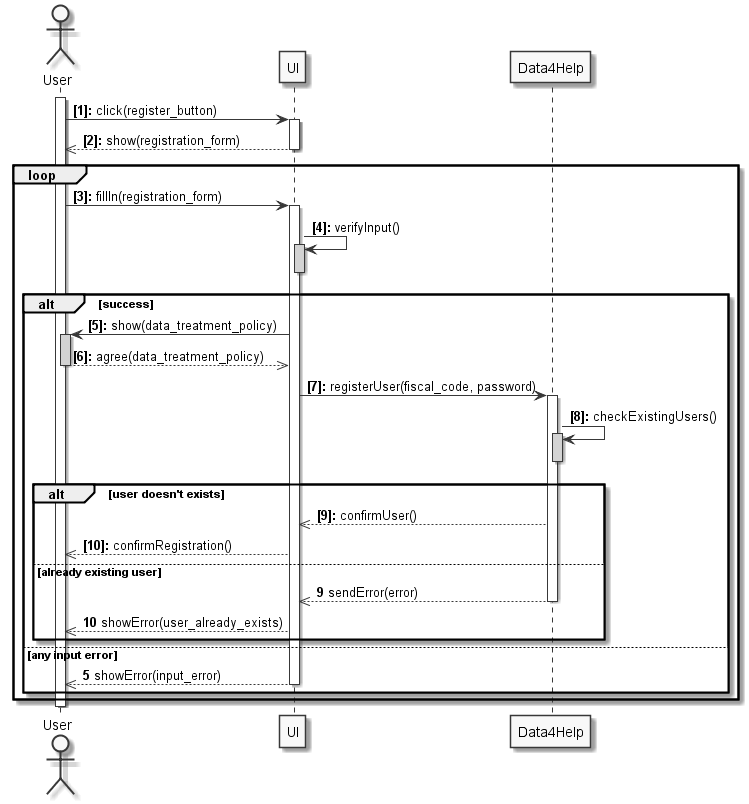
\includegraphics[width=\linewidth]{seq_user_registration.png}
	\caption{Data4Help - User Registration Sequence}
	\label{Data4Help - User Registration Sequence}
\end{figure}

\begin{figure}
	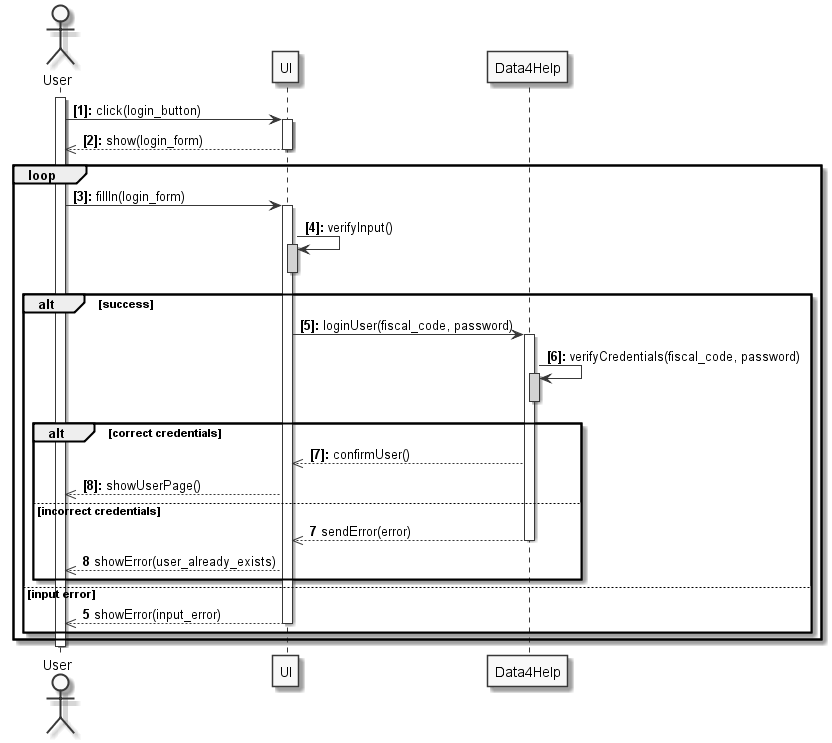
\includegraphics[width=\linewidth]{seq_user_login.png}
	\caption{Data4Help - User Login Sequence}
	\label{Data4Help - User Login Sequence}
\end{figure}

\begin{figure}
	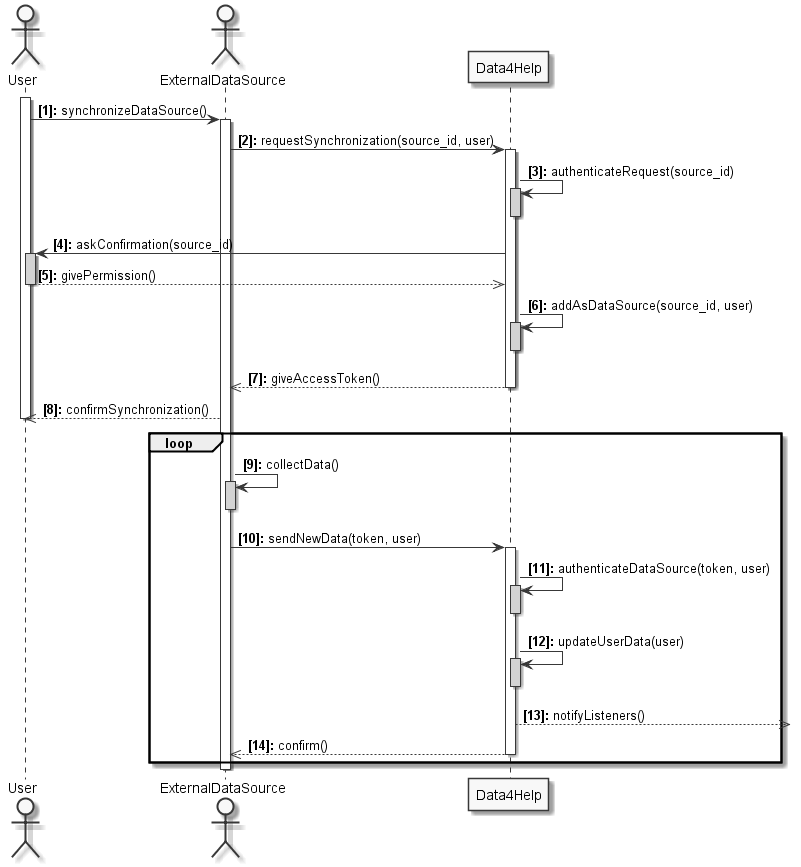
\includegraphics[width=\linewidth]{seq_new_datasource.png}
	\caption{Data4Help - Data Source Synchronization Sequence}
	\label{Data4Help - Data Source Synchronization Sequence}
\end{figure}                                           

\begin{figure}
	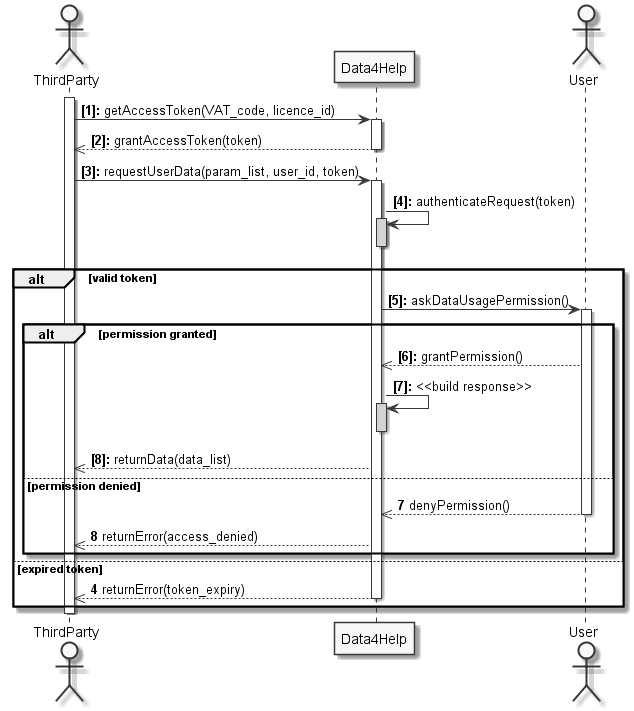
\includegraphics[width=\linewidth]{seq_thirdparty_singledata_req.png}
	\caption{Data4Help - Third Party single data request sequence}
	\label{Data4Help - Third Party single data request sequence}
\end{figure}

\begin{figure}
	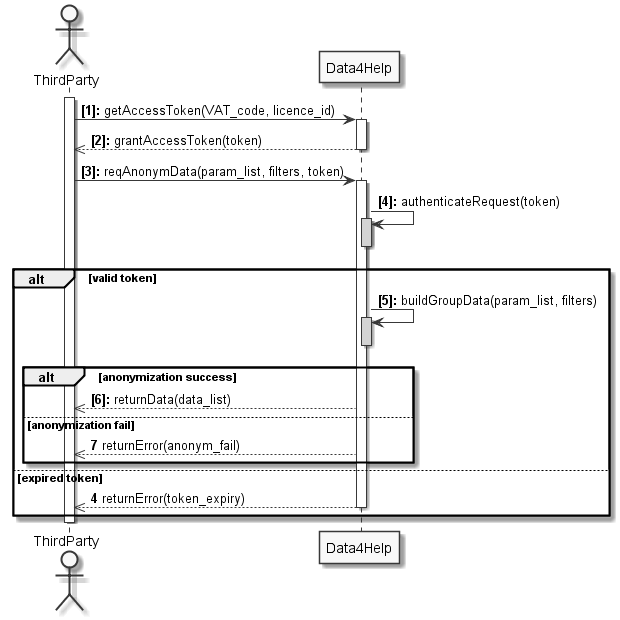
\includegraphics[width=\linewidth]{seq_thirdparty_singleanonym_req.png}
	\caption{Data4Help - Third Party group data request sequence}
	\label{Data4Help - Third Party group data request sequence}
\end{figure}  

\begin{figure}
	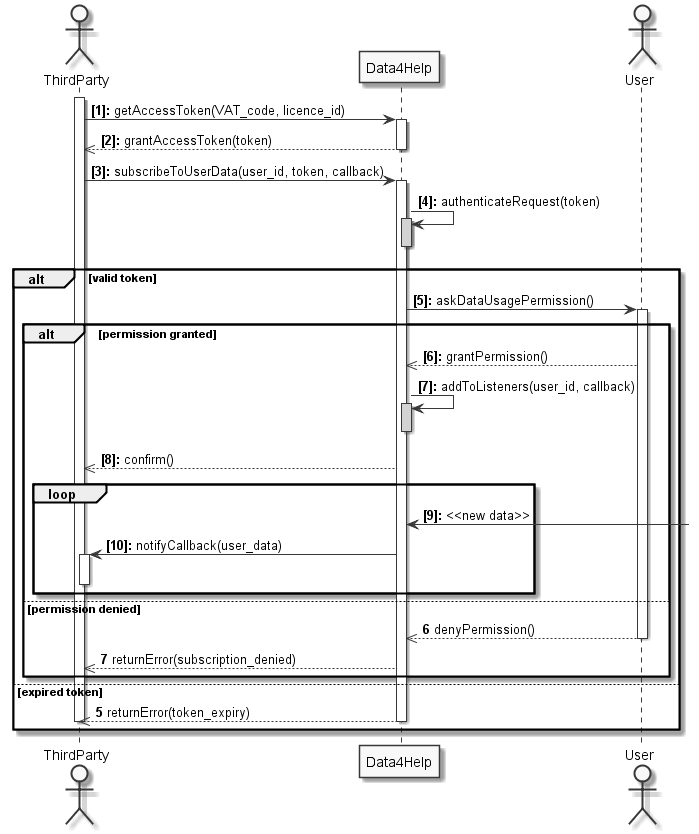
\includegraphics[width=\linewidth]{seq_thirdparty_subscription.png}
	\caption{Data4Help - Third Party subscription request sequence}
	\label{Data4Help - Third Party subscription request sequence}
\end{figure}

\FloatBarrier
\textbf{AutomatedSOS Sequence Diagrams}

\begin{figure}[H]
	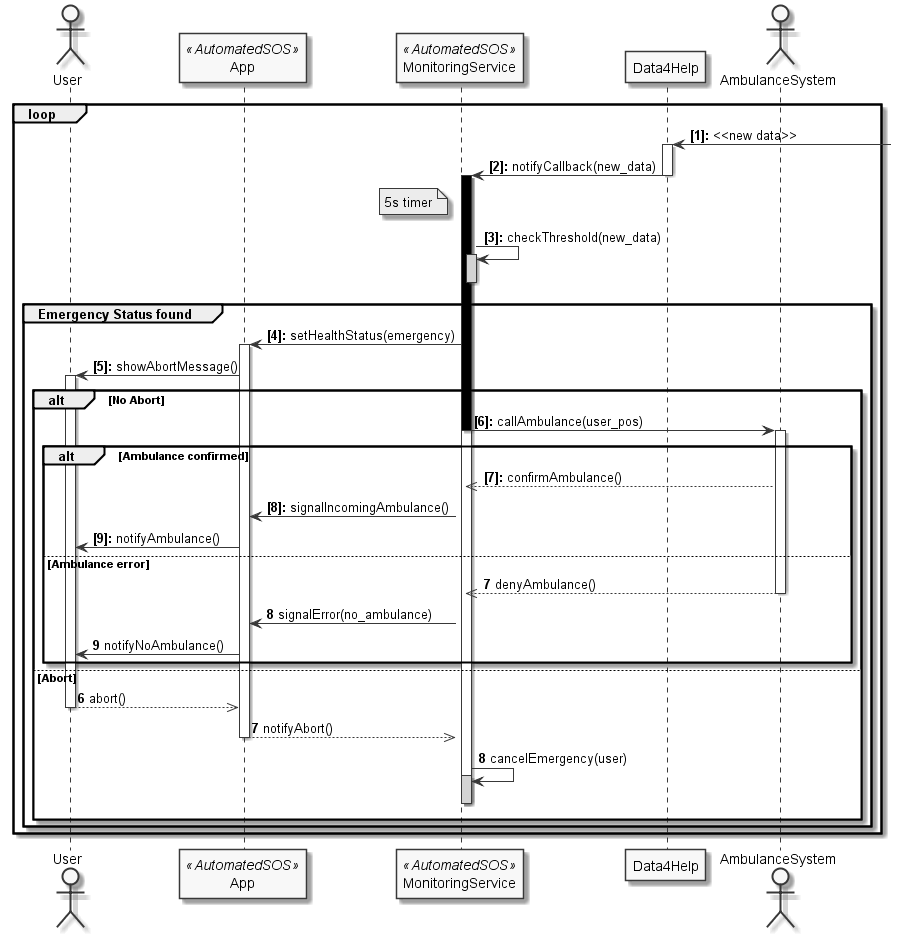
\includegraphics[width=\linewidth]{seq_sos_emergency.png}
	\caption{AutomatedSOS - Emergency sequence}
	\label{AutomatedSOS - Emergency sequence}
\end{figure}                

\begin{figure}
	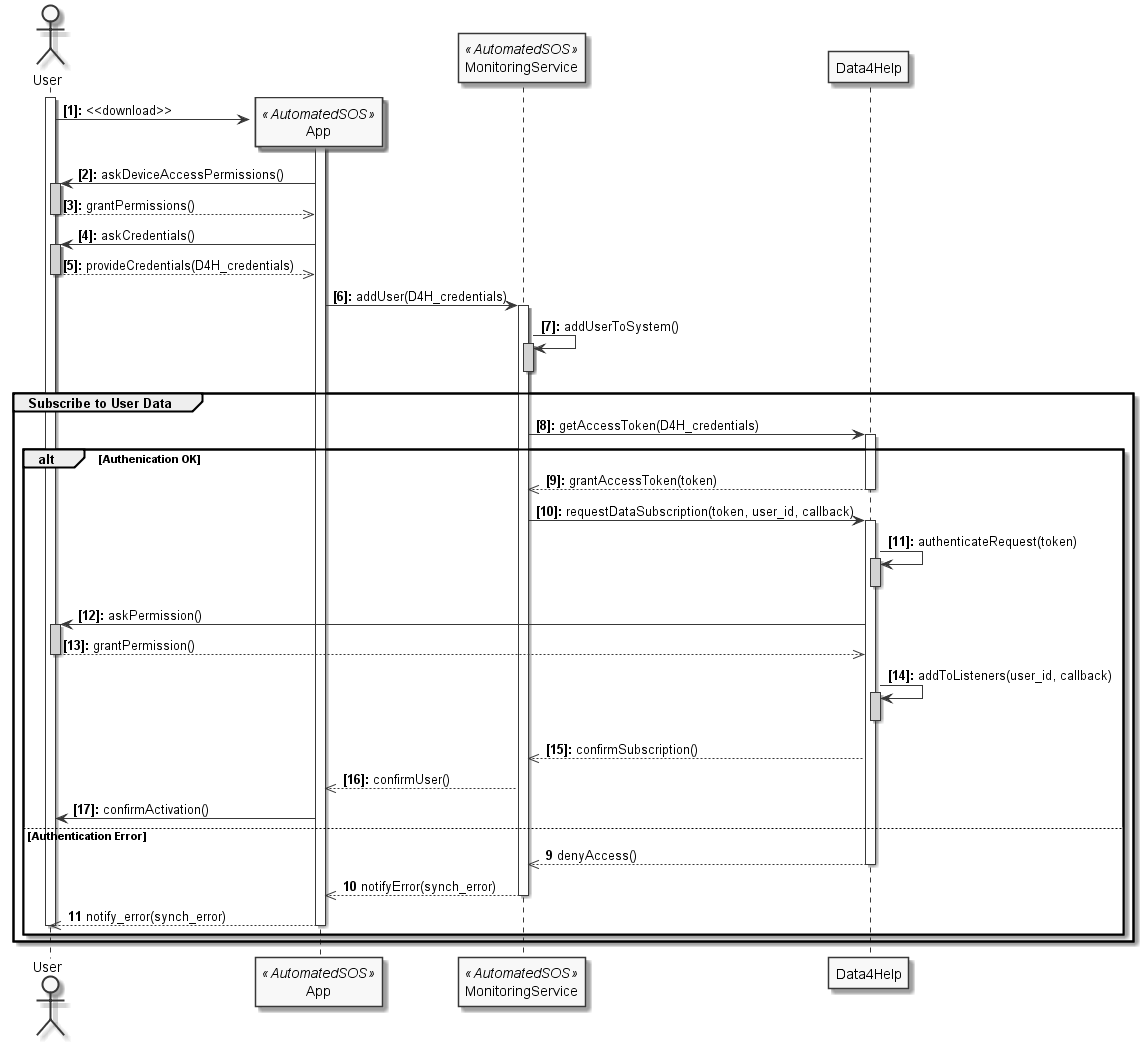
\includegraphics[width=\linewidth]{seq_sos_registration.png}
	\caption{AutomatedSOS - User Registration sequence}
	\label{AutomatedSOS - User Registration sequence}
\end{figure} 

\FloatBarrier
\textbf{Track4Run Sequence Diagrams}

\begin{figure}[H]
	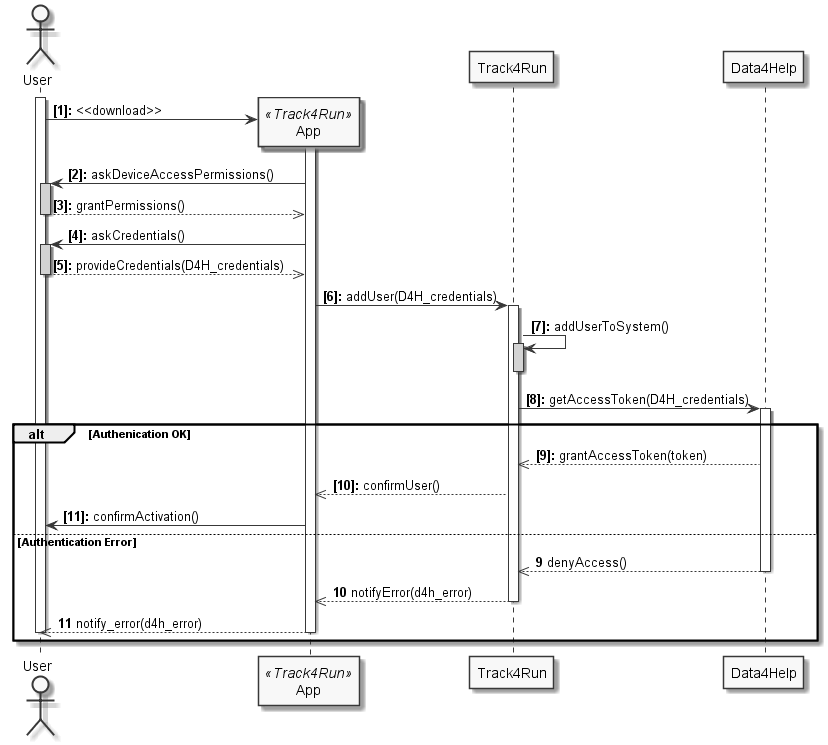
\includegraphics[width=\linewidth]{t4r_reg.png}
	\caption{Track4Run - User Registration sequence}
	\label{Track4Run - User Registration sequence}
\end{figure}

\begin{figure}
	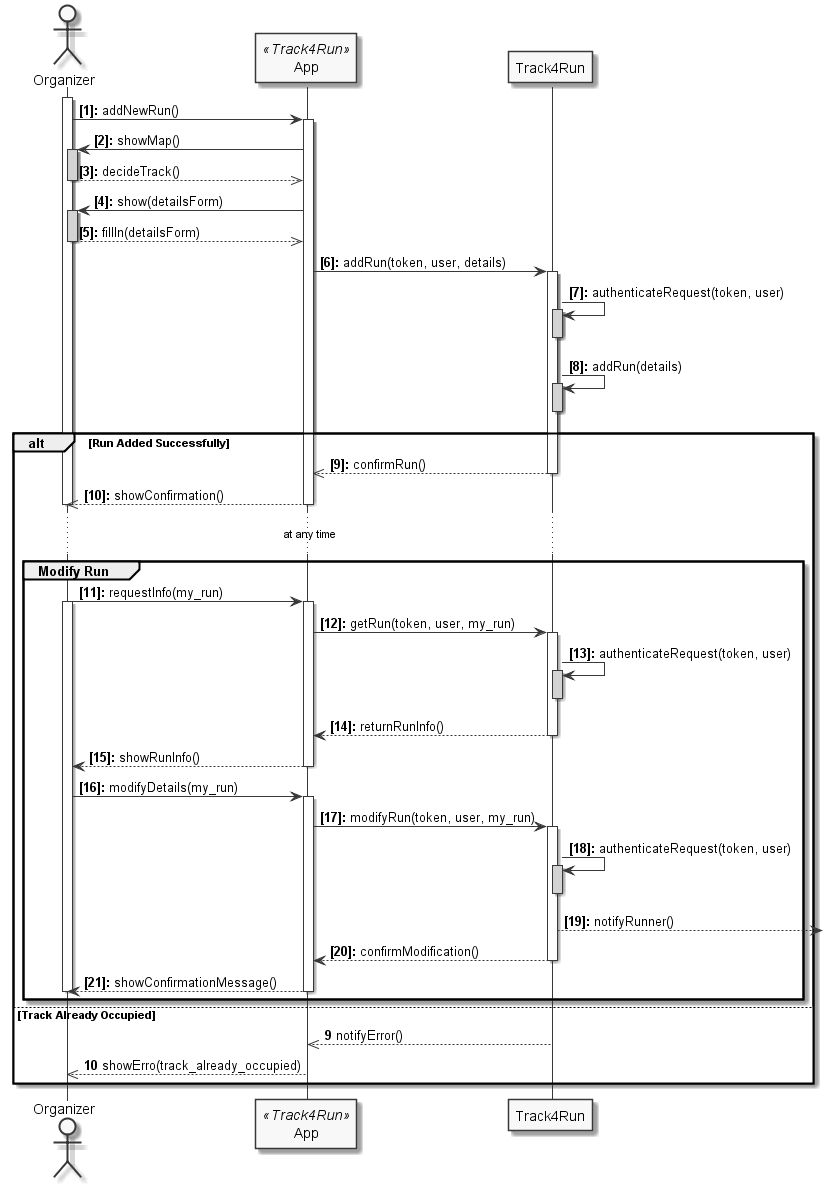
\includegraphics[width=\linewidth]{t4r_new_run.png}
	\caption{Track4Run - Run Creation sequence}
	\label{Track4Run - Run Creation sequence}
\end{figure}

\begin{figure}
	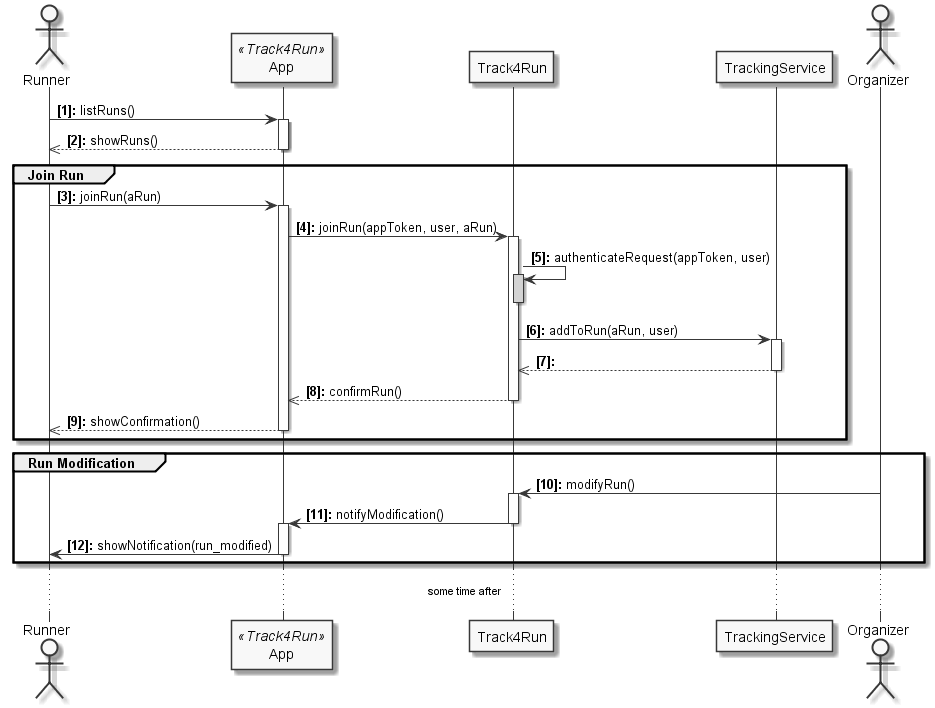
\includegraphics[width=\linewidth]{t4r_join_run.png}
	\caption{Track4Run - Run joining sequence}
	\label{Track4Run - Run joining sequence}
\end{figure}

\begin{figure}
	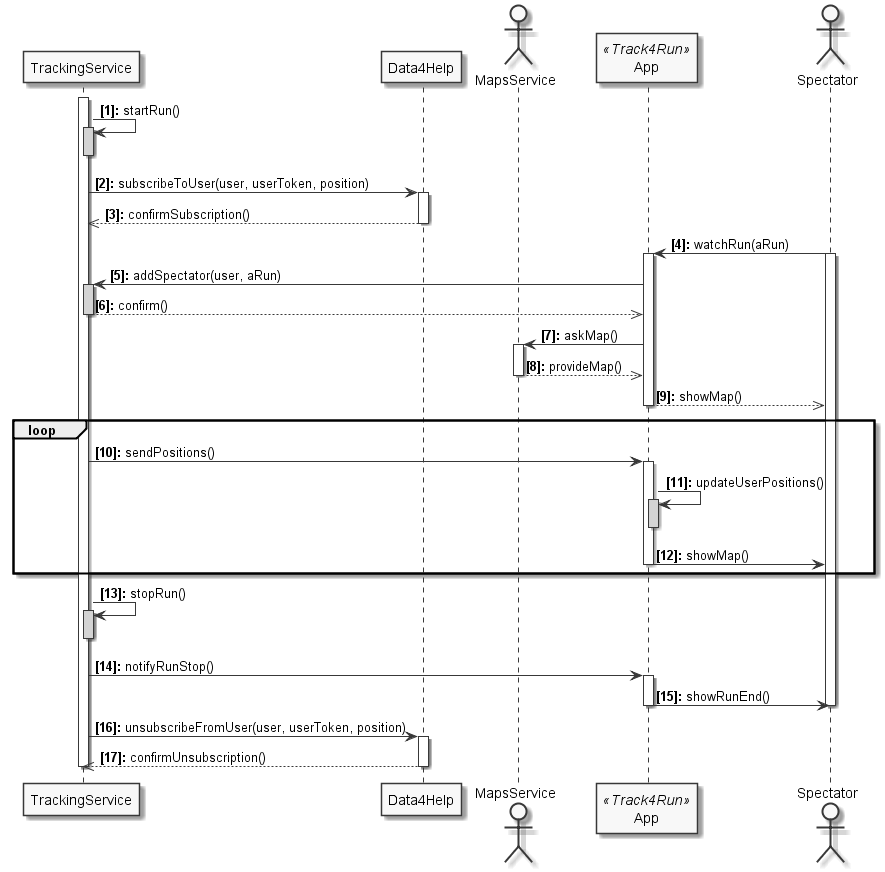
\includegraphics[width=\linewidth]{t4r_watch_run.png}
	\caption{Track4Run - Spectator watching run sequence}
	\label{Track4Run - Spectator watching run sequence}
\end{figure}
\FloatBarrier

\subsection{Performance Requirements}
In general, the main performance requirements for our system concern the time needed to process data and fulfill data requests.

In particular, the system should meet the following strong requirement:

\begin{itemize}
	\item \textbf{AutomatedSOS Emergency Response}
	The system must call an ambulance within \textbf{5 seconds} from when a parameter exceeds a threshold. This time shall take into account the time needed for the AutomatedSOS monitoring system to process new incoming data and detect the emergency, the Data4Help system to send the new data to AutomatedSOS and the average delay introduced from the communication interfaces.
\end{itemize}

\subsection{Design Constraints}
\subsubsection{Regulatory policies}
\begin{itemize}
	\item \textbf{GDPR}: In order to protect the user's privacy and perform a correct data treatment, the system must be developed in compliance with the latest GDPR regulations, giving the maximum attention to the protection and anonymization of the user's data.
\end{itemize}
\subsubsection{Hardware limitations}
The only hardware limitations of our system is present in the devices on which AutomatedSOS and Track4Run applications will be installed. For this reason, the development of the software to be will have to reasonably take in account some common limitations of these devices, such as power consumption and memory size.


\subsection{Software System Attributes}
\subsubsection{Reliability}

The system must be available 24/7. Since this requirement is quite demanding, small service breaks will be tolerated. To boost reliability, a RAID architecture that combines multiple disk drives to have data redundancy is suggested. Using a RAID controller we could also expand disks' capacity or substitute them without the risk of losing data or suspending the service for too long. Preventive maintenance is also a good idea to avoid downtimes.

\subsubsection{Availability}

To guarantee a 3-nines (99.9\%) availability degree, a system of redundant servers could be considered. In this way we don't have a single point of failure and if one server fails, another one will be ready to substitute it.

\subsubsection{Security}

Security is a main issue.  At first, to access the functionalities offered by our platform, users have to complete a login phase providing their credentials: fiscal code and password in case of a single user or VAT code and electronic signature for the third parties. These sensitive information should be confidentially stored and encrypted using a proper hash function.

Secondly, the system  continuously collects data on health conditions from the users. Typically this kind of data are also considered sensitive and should be kept secret. Finally, also communications between users and our platform is very important, for this reason the system could be accessed by the customers using secure connection protocols like HTTPS to avoid Man In The Middle attacks. Only the system administrator who is responsible of the Web and Application Server configuration can decide if it is the case to implement them or not.

\subsubsection{Maintainability}

In order to make our software the most maintainable as possible, we will adopt a modular design for our code. In this different components of the system can be modified and additional ones can be introduced in the system with whenever is needed and with a minimal impact on the rest of the system.

Moreover, we will make sure to adopt standard design patterns and coding best practices, so that our code can be easily understood and modified by any future developer.

Finally, the code should be completely and properly documented in order to facilitate the understanding of it. 

\subsubsection{Portability}

During the system installation and setup, we have to consider different factors:

\begin{itemize}
	\item Ease of installation on the central server
	\item Scalability of the platform considering future adjustments without losing the already collected data
	\item Portability of data between different machines, in order to move the system on several more powerful machines in case of necessity
	up 24/7
\end{itemize}
